% compile with XeLaTeX or LuaLaTeX
\documentclass[10pt,a5paper,twoside]{article}
\usepackage{iftex}
\RequireXeTeX
\usepackage[top=12mm,bottom=26mm,outer=28mm,inner=14mm,foot=14mm]{geometry}
\usepackage{calc}
\usepackage{scrextend}
\deffootnote[1.5em]{0em}{1em}{\thefootnotemark\quad}
\renewcommand{\footnoterule}{%
  \kern -2.4pt
  \hrule width \textwidth height 0.4pt
  \kern 2pt
}

\usepackage{fontspec}
\setmainfont[
	Ligatures=TeX,
	Extension=.otf,
	SlantedFont=cmunsl,
	BoldFont=cmunbx,
	ItalicFont=cmunti,
	BoldItalicFont=cmunbi,
	SmallCapsFont=cmunrm, % for upright instead of slanted small caps
	SmallCapsFeatures={Letters=SmallCaps,Numbers=OldStyle},	
]{cmunrm}

\usepackage{etoolbox}
\usepackage{microtype,ellipsis}

\usepackage{polyglossia,iflang}
\setotherlanguage{russian} % the name of the original Russian version at the end of this book is written using Cyrillic letters

\usepackage{textcomp}

\usepackage{amsmath,amssymb,nicefrac,amscd}
\usepackage{graphicx,float}
\usepackage{import}
\usepackage{pdfpages}

\usepackage{enumitem}
\setitemize[1]{noitemsep,nosep,leftmargin=0.99em,label={--}}

\usepackage{transparent}
\usepackage{csquotes}
\DeclareQuoteStyle{vietnamese}
  {\textquotedblleft}
  {\textquotedblright}
  [0.05em]
  {\textquoteleft}
  {\textquoteright}

\usepackage{siunitx}
\sisetup{per-mode=fraction,fraction-function=\nicefrac}

\usepackage{hyperref}

\usepackage{todonotes}

\newcommand{\eps}{\varepsilon}

% Usually, you would define a theorem-like enviroment which uses automatic numbering
% but Arnold also uses special numbering for some problems. Therefore, I kept the manual numbering.
\newenvironment{problem}[1]{\paragraph*{#1}}{}

\newenvironment{note}[1]{\par\noindent\IfLanguageName{vietnamese}{\textit{#1}}{\textsc{\MakeLowercase{#1}}} }{\par}

\makeatletter

% do no indent the first paragraph of the abstract
\let\oldabstract\abstract
\def\abstract{\oldabstract\noindent\@ifnextchar\par{\expandafter\abstract\@gobble}{}}

% always center contents of floats
\g@addto@macro\@floatboxreset{\centering}

% make all figures use 'H' position by default:
\def\fps@figure{H}
\makeatother

\setdefaultlanguage[variant=british]{english}

\title{Problems for children from 5 to 15}

\author{V.\,I.~Arnold
\vspace*{2cm}\\ 
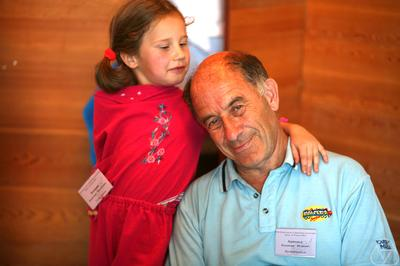
\includegraphics[width=\linewidth]{photo-arnold_small}
}
\date{}

\begin{document}
\maketitle
\thispagestyle{empty}
\cleardoublepage 
\setcounter{page}{1}
\begin{abstract}
This brochure consists of 77 problems for development of thinking culture, either selected or composed by the author.
Most of them do not require any special knowledge beyond the general education. However, solving some of them may
turn out challenging even for professors.

The book is addressed to school and university students, teachers, parents -- to everybody who considers the thinking culture 
an essential part of the personality development.
\end{abstract}
\clearpage 

\section*{Preface}
I put these problems onto paper in Paris in spring 2004 when Russian Parisians asked me to help
their young children gain the thinking culture traditional for Russia.

I am deeply convinced that this culture is most of all cultivated by early independent reflection
on simple, but not easy questions similar to those below (problems 1, 3, 13 are the most recommended).

My long experience has shown that, very frequently, dimwits falling at school behind solve them better
than A-grade pupils, since -- for their survival at the back of the classroom -- they must permanently
think more than required \enquote{for governing the whole Seville and Granada}, as Figaro used to say about
himself, while A-graders cannot catch \enquote{what should be multiplied by what} in these problems.

I have also noticed that five year old kids solve similar problems better than pupils spoiled
by coaching, which in their turn cope with the questions better than university students used
to swotting who anyway beat their professors (the worst in solving these simple problems are
Nobel and Fields prize winners).   

\clearpage
\section*{The problems}

\begin{problem}{1.}
	Masha was seven kopecks short to buy a first reading book, and Misha lacked one kopeck.
	They combined their money to buy one book to share, but even then they did not have enough.
	How much did the book cost?
\end{problem}

\begin{problem}{2.}
	A bottle with a cork costs 10 kopecks, while the bottle itself is 9 kopecks more expensive
	than the cork. How much does the bottle without the cork cost?
\end{problem}

\begin{problem}{3.}
	A brick weighs one pound and half the brick. How many pounds does the brick weigh?
\end{problem}

\begin{problem}{4.}
	A spoon of wine is poured from a barrel of wine into a (not full) glass of tea.
	After that, the same spoon of the (inhomogeneous) mixture from the glass is taken back into the barrel.
	Now both in the barrel and in the glass there is a certain volume of the foreign liquid (wine in the glass and
	tea in the barrel). In which is the volume of the foreign liquid greater: in the glass or in the barrel?
\end{problem}

\begin{problem}{5.}
	Two old ladies left from $A$ to $B$ and from $B$ to $A$ at dawn
	heading towards one another (along the same road). They met at noon,
	but did not stop, and each of them carried on walking with the same speed.
	The first lady came (to $B$) at 4\,p.m., and the second (to $A$) at 9\,p.m. What time was the dawn that day? 
\end{problem}

\begin{problem}{6.}
	The hypotenuse of a right-angled triangle (in a standard American examination) is 10~inches,
	the altitude dropped onto it is 6~inches. Find the area of the triangle.

	American school students had been coping successfully with this problem over a decade.
	But then Russian school students arrived from Moscow, and none of them was able to solve it as had their American peers
	(giving 30~square inches as the answer). Why? 
\end{problem}

\begin{problem}{7.}
	Vasya has 2 sisters more than he has brothers. How many daughters more than sons do Vasya's parents have?
\end{problem}

\begin{problem}{8.}
	There is a round lake in South America. Every year, on June~1, a Victoria Regia flower appears at its
	centre (its stem rises from the bottom, and its petals lie on the water like those of a water lily). Every day
	the area of the flower doubles, and on July~1, it finally covers the entire lake, drops its petals, and its seeds
	sink to the bottom. On which date is the flower's area half the area of the lake?    
\end{problem}

\begin{problem}{9.}
	A peasant must take a wolf, a goat and a cabbage across a river in a boat. However the boat is so small that
	he is able to take only one of the three on board with him. How should he transport all three across
	the river? (The wolf cannot be left alone with the goat, and the goat cannot be left alone with the cabbage.)
\end{problem}

\begin{problem}{10.}
	During the daytime a snail climbs \SI{3}{\cm} up a post, and during the night, falling asleep, accidentally
	goes down by \SI{2}{\cm}. The post is \SI{10}{\metre} high, and a delicious (for the snail) sweet is on its top.
	In how many days will the snail get the sweet?
\end{problem}

\begin{problem}{11.}
	A ranger walked from his tent \SI{10}{\km} southwards, turned east, walked straight eastwards \SI{10}{\km} more,
	met his bear friend, turned north and after another \SI{10}{\km} found himself by his tent. What colour was the bear
	and where did all this happen?
\end{problem}

\begin{problem}{12.}
	A tide was in today at 12~noon. What time will it be in (at the same place) tomorrow?
\end{problem}

\begin{problem}{13.}
	Two volumes of Pushkin, the first and the second, are side-by-side on a bookshelf. The pages of each
	volume are \SI{2}{\cm} thick, and the cover -- front and back each -- is \SI{2}{\mm}. A bookworm has gnawed through
	(perpendicular to the pages) from the first page of volume~1 to the last page of volume~2. How long is the bookworm's track? [This topological problem with an incredible answer \SI{4}{\mm} is absolutely impossible for academicians,
	but some preschoolers handle it with ease.]
\end{problem}

\begin{problem}{14.}
	Find a body with views from the top and from the front as depicted (polytopes).
	Depict its side view (showing invisible edges of the polytope dashed).
	\begin{figure}
		\footnotesize
		\null\hfill
		\parbox{0.2\linewidth}{\centering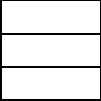
\includegraphics{taskbook-99}\\Top view}
		\hfill
		\parbox{0.2\linewidth}{\centering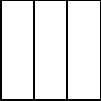
\includegraphics{taskbook-98}\\Front view}
		\hfill\null
	\end{figure}
\end{problem}

\begin{problem}{15.}
	How many ways are there to break up the number 64 into 10 positive integer summands, whose maximum is 12? [Ways that differ only by the order of their summands do not count as different.]
\end{problem}

\begin{problem}{16.}
	By putting a few similar bars one onto another (for example, domino pieces),
	one can make a length $x$ overhang. What is the maximal attainable value of the overhang length $x$?
	\begin{figure}
		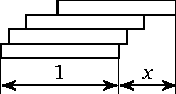
\includegraphics{taskbook-97}
	\end{figure}
\end{problem}

\begin{problem}{17.}
	The distance between cities $A$ and $B$ is \SI{40}{\km}. Two cyclists leave respectively from $A$ and $B$ simultaneously
	towards one another, one with speed \SI{10}{\km\per\hour} and the other with speed \SI{15}{\km\per\hour}. A fly flies out with the first
	cyclist from $A$ with the speed of \SI{100}{\km\per\hour}, reaches the second, touches his forehead and flies back to the first,
	touches his forehead, returns to the second, and so on until the cyclists' foreheads collide and squash
	the fly.
	How many kilometres altogether has the fly flown?
	\begin{figure}
		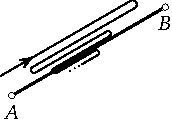
\includegraphics{taskbook-1}
	\end{figure}
\end{problem}

\begin{problem}{18.}
	One domino piece covers two squares of a chessboard. 
	Cover all the squares
	except for two opposite ones (on the same diagonal) with 31 pieces. [A chessboard consists of $8 \times 8 = 64$ squares.]
	\begin{figure}
		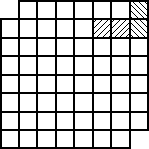
\includegraphics{taskbook-2}
	\end{figure}
\end{problem}

\begin{problem}{19.}
	A caterpillar wants to slither from a corner of a cubic room (the left on the floor) to the opposite one
	(the right on the ceiling).
	Find the shortest route for such a journey along the walls of the room.
	\begin{figure}
		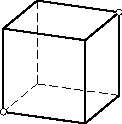
\includegraphics{taskbook-3}
	\end{figure}
\end{problem}

\begin{problem}{20.}
	You have two vessels of volumes 5~litres and 3~litres. Measure out one litre (obtaining it in one of the vessels).
	\begin{figure}
		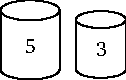
\includegraphics{taskbook-4}
	\end{figure}
\end{problem}

\begin{problem}{21.}
	There are five heads and fourteen legs in a family. How many people and how many dogs are in the family?
\end{problem}

\begin{problem}{22.}
	Equilateral triangles are constructed externally on sides $AB$, $BC$ and $CA$ of a triangle $ABC$.
	Prove that their centres ($*$) form an equilateral triangle.
	\begin{figure}
		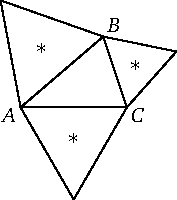
\includegraphics{taskbook-6}
	\end{figure}
\end{problem}

\begin{problem}{23.}
	What polygons may be obtained as sections of a cube by a plane? Can we get a pentagon? A heptagon?
	A regular hexagon?
	\begin{figure}
		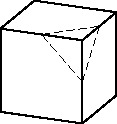
\includegraphics{taskbook-7}
	\end{figure}
\end{problem}

\begin{problem}{24.}
	Draw a straight line through the centre of a cube so that the sum of squares of the distances to it
	from the eight vertices of the cube would be
	a) maximal,
	b) minimal (comparing with other such lines).
\end{problem}

\begin{problem}{25.}
	A right circular cone is cut by a plane along a closed curve. Two balls inscribed into the cone
	are tangent to the plane, one at point $A$ and the other at point $B$. Find a point $C$ on the cut line so
	that the sum of the distances $CA + CB$ would be a) maximal, b) minimal.
	\begin{figure}
		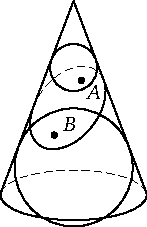
\includegraphics{taskbook-9}
	\end{figure}
\end{problem}

\begin{problem}{26.}
	The Earth's surface is projected onto the cylinder formed by the lines tangent to the meridians
	at their equatorial points along the rays parallel to the equator and passing through the Earth's pole axis.
	Will the area of the projection of France be greater or smaller than the area of France itself?
	\begin{figure}
		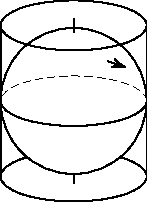
\includegraphics{taskbook-10}
	\end{figure}
\end{problem}

\begin{problem}{27.}
	Prove that the remainder of division of the number $2^{p-1}$ by an odd prime $p$ is $1$.
	(Examples: $2^2 = 3a + 1$, $2^4 = 5b+1$, $2^6 = 7c+1$, $2^{10} - 1 = 1023 = 11\cdot 93$.)  
\end{problem}

\begin{problem}{28.}
	A needle \SI{10}{\cm} long is thrown randomly onto lined paper with the distance between neighbouring
	lines also \SI{10}{\cm}. This is repeated
	$N$ (a million) times. 
	How many times (approximately, up to a few per
	cent error) will the fallen needle intersect a line on the paper?
	\begin{figure}
		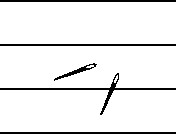
\includegraphics[scale=1]{taskbook-12}
	\end{figure}
	One can perform (as I did at the age of 10) this experiment with $N=100$ instead of a million throws.
	[The answer to this problem is surprising: $\frac2{\pi}N$. Moreover even for a bent needle of length $a \cdot \SI{10}{\cm}$ the number of intersections observed over $N$ throws will be approximately $\frac{2a}{\pi}N$. 
	The number $\pi \approx  \frac{355}{113} \approx \frac{22}7.$]
\end{problem}

\begin{problem}{29.}
	Polyhedra with triangular faces are, for example, Platonic solids: tetrahedron (4 faces),
	octahedron (8 of them), icosahedron (20 -- and all the faces are the same; it is interesting to draw it,
	it has 12 vertices and 30 edges).
	\begin{figure}
		\footnotesize
		\null\hfill
		\parbox{0.3\linewidth}{\centering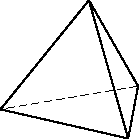
\includegraphics{taskbook-131}\\Tetrahedron ($\text{tetra}= 4$)}
		\hfill
		\parbox{0.3\linewidth}{\centering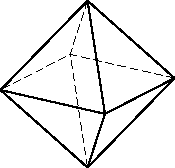
\includegraphics{taskbook-132}\\Octahedron ($\text{octo}= 8$)}
		\hfill\null\\
		{\Huge ?}\\Icosahedron
	\end{figure}
	Is it true that for any such (bounded convex polyhedron with triangular faces) the number of faces is
	equal to twice the number of vertices minus four?


	Yet another Platonic solid (there are 5 of them altogether):
	\begin{figure}
		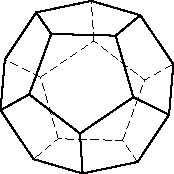
\includegraphics{taskbook-14}
	\end{figure}
\end{problem}

\begin{problem}{30.}
	A dodecahedron is a convex polyhedron with twelve (regular) pentagonal
	faces, twenty vertices
	and thirty edges (its vertices are the centres of the faces of an icosahedron).
	Inscribe into a dodecahedron five cubes (the vertices of each cube are vertices of the dodecahedron)
	whose edges are diagonals of faces of the dodecahedron (a cube has 12~edges, one per face).
	[This was invented by Kepler for the sake of planets.] 
\end{problem}

\begin{problem}{31.}
	Find the intersection of two tetrahedra inscribed into a cube (so that the vertices of each are
	vertices of the cube, and the edges are diagonals of the faces). 
	What fraction of the cube's volume is contained within the tetrahedra's intersection?
\end{problem}

\begin{problem}{31\textsuperscript{bis}.}
	Construct the section of a cube by the plane passing through three given points on the edges.
	[Draw the polygon along which the planar section intersects the faces of the cube.]
	\begin{figure}
		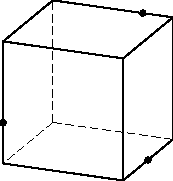
\includegraphics{taskbook-15}
	\end{figure}
\end{problem}

\begin{problem}{32.}
	How many symmetries does a tetrahedron have? How many has a cube? octahedron? icosahedron?
	dodecahedron? A symmetry is a transformation preserving lengths.
	How many rotations are among them and how many reflections (in each of the five cases listed)?
\end{problem}

\begin{problem}{33.}
	How many ways are there to paint $6$ faces of similar cubes with six colours $(1,\dotsc,6)$ [one per face]
	so that no two of the coloured cubes obtained would be the same (could not be transformed one into another
	by a rotation)? 
	\begin{figure}
		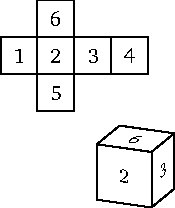
\includegraphics{taskbook-17}
	\end{figure}
\end{problem}

\begin{problem}{34.}
	How many different ways are there to permute $n$ objects?
	There are six of them for $n=3$: $(1,2,3)$, $(1,3,2)$, $(2,1,3)$, $(2,3,1)$, $(3,1,2)$, $(3,2,1)$. What if the number of objectis is $n=4$? $n=5$? $n=6$? $n=10$?
	\begin{figure}
		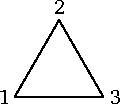
\includegraphics{taskbook-18}
	\end{figure}
\end{problem}

\begin{problem}{35.}
	A cube has $4$ long diagonals. How many different permutations of these four objects are obtained by rotations of a cube?
	\begin{figure}
		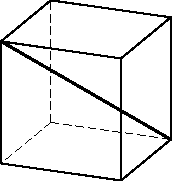
\includegraphics{taskbook-19}
	\end{figure}
\end{problem}

\begin{problem}{36.}
	The sum of the cubes of three integers is subtracted from the cube of the sum of these numbers. Is the difference always divisible by $3$?
\end{problem}

\begin{problem}{37.}
	Same question for the fifth powers and divisibility by $5$, and for the seventh powers and divisibility by $7$.
\end{problem}

\begin{problem}{38.}
	Calculate the sum
	\begin{equation*}
		\frac{1}{1\cdot 2} + \frac{1}{2\cdot 3} + \frac{1}{3\cdot 4} + \dotsb + \frac{1}{99\cdot 100}
	\end{equation*}
	(with an error of not more than $1\%$ of the answer).
\end{problem}

\begin{problem}{39.}
	If two polygons have equal areas, then they may be cut into a finite number of polygonal parts which may then be rearranged to obtain both the first and second polygons. Prove this! [For spatial solids this is not the case: the cube and tetrahedron of equal volumes cannot be cut this way!]
	\begin{figure}
		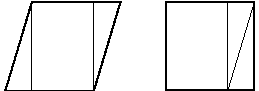
\includegraphics{q39_horizontal}
	\end{figure}
\end{problem}

\begin{problem}{40.}
	Four vertices of a parallelogram have been chosen at nodes of a piece of squared paper. It turns out that neither the parallelogram's sides nor its interior contain any other nodes of the squared paper. Prove that the area of such a parallelogram is equal to the area of one square of the paper. 
	\begin{figure}
		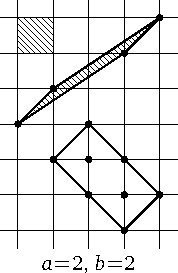
\includegraphics{taskbook-24}
	\end{figure}
\end{problem}

\begin{problem}{41.}
	Under the conditions of question 40, $a$ nodes have turned out to be in the interior and $b$ on the sides of the parallelogram. Find its area. 
\end{problem}

\begin{problem}{42.}
	Is the statement analogous to question 40 true for parallelepipeds in 3-space?
\end{problem}

\begin{problem}{43.}
	The rabbit (or Fibonacci) numbers form a sequence $1,2,3,5,8,\allowbreak 13,21,34,\dotsc$, in which $a_{n+2}=a_{n+1}+a_n$ for any
	$n=1,2,\dotsc$ ($a_n$ is the $n$-th number in the sequence). Find the greatest common divisor of the numbers $a_{100}$ and $a_{99}$.
\end{problem}

\begin{problem}{44.}
	Find the (Catalan) number of ways to cut a convex $n$-gon into triangles by cutting along its non-intersecting diagonals. 
	For example, $c(4)=2$, $c(5)=5$, $c(6)=14$. How can one find $c(10)$?
	\begin{figure}
		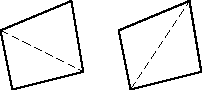
\includegraphics{taskbook-281}
		\qquad
		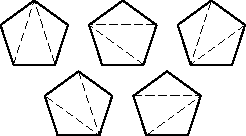
\includegraphics{taskbook-282}
	\end{figure}
\end{problem}

\begin{problem}{45.} 
	A cup tournament has $n$ participating teams, each losing team leaves, and the overall winner is decided after $n-1$ games.
	The tournament schedule may be written symbolically as, for instance,  $((a,(b,c)),d)$ meaning $b$ plays $c$, the winner meets $a$, and the winner of those meets $d$].
	What is the number of different schedules for 10 teams? 
	\begin{itemize}
		\item For 2 teams, we have only $(a,b)$, and the number is 1.
		\item For 3 teams, there are only $((a,b),c)$, or $((a,c),b)$, or $((b,c),a)$, and the number is 3.
		\item For 4 teams:
			\begin{equation*}
				\begin{array}{@{}cccc@{}}
					(((a,b),c),d) & \quad\;(((a,c),b),d) & \quad\;(((a,d),b),c) & \quad\;(((b,c),a),d) \\
					(((b,d),a),c) & \quad\;(((c,d),a),b) & \quad\;(((a,b),d),c) & \quad\;(((a,c),d),b) \\ 
					(((a,d),c),b) & \quad\;(((b,c),d),a) & \quad\;(((b,d),c),a) & \quad\;(((c,d),b),a) \\
					((a,b),(c,d)) & \quad\;((a,c),(b,d)) & \quad\;((a,d),(b,c))
				\end{array}
			\end{equation*}
	\end{itemize}
\end{problem}

\begin{problem}{46.}
	Join $n$ points $1, 2, \dotsc, n$ by intervals ($n-1$ of them) to obtain a tree. How many different trees may be obtained (the $n=5$ case is already interesting!)?
	 
	$n=2$:\quad 
\includegraphics{taskbook-291}\,,\quad the number is 1; 

	$n=3$:\quad 
	
\includegraphics{taskbook-292}\,,\quad 
	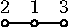
\includegraphics{taskbook-293}\,,\quad 
	
\includegraphics{taskbook-294}\,,\quad 
	the number is 3;

	$n=4$:\quad\def\quad{\hskip.7em}
	$\vcenter{\hbox{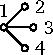
\includegraphics{taskbook-295}}}$,\quad
	$\vcenter{\hbox{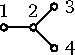
\includegraphics{taskbook-296}}}$,\quad
	$\vcenter{\hbox{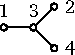
\includegraphics{taskbook-297}}}$,\quad
	$\vcenter{\hbox{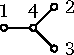
\includegraphics{taskbook-298}}}$,\quad
	$\vcenter{\hbox{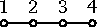
\includegraphics{taskbook-299}}\hbox{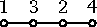
\includegraphics{taskbook-290}}
	\vskip-8pt
	\hbox to50bp{\dotfill}}$,\\
	\null\hspace{\parindent}\phantom{$n=4$:}\quad the number is 16.
\end{problem}

\begin{problem}{47.}
	A permutation $(x_1,x_2, \dotsc,x_n)$ of numbers $\{1, 2, \dotsc, n\}$ is called a 
    \emph{snake} (of length $n$) if $x_1<x_2>x_3<x_4 \dotsb$.

	\begin{note}{Example:}
		\begin{equation*}
			\begin{aligned}[t]
				&\begin{aligned}[t] n=2, \text{\ \ only\ \ } 1<2, \end{aligned} &&\text{the number is }1, \\
				&\hskip-\nulldelimiterspace\mathord{\left.\begin{aligned} n=3, \hphantom{\text{\ \ only\ \ }} 1&<3>2 \\ 
				2&<3>1\end{aligned} \right\}}, && \text{the number is }2, \\
				&\hskip-\nulldelimiterspace\mathord{\left.\begin{aligned} n=4, \hphantom{\text{\ \ only\ \ }} 1&<3>2<4 \\ 
				1&<4>2<3 \\ 
				2&<3>1<4 \\ 
				2&<4>1<3 \\ 
				3&<4>1<2\end{aligned} \right\}},
				&&\text{the number is }5. \\
			\end{aligned}
		\end{equation*}
	\end{note}
	Find the number of snakes of length $10$.
\end{problem}

\begin{problem}{48.}
	Let $s_n$ be the number of snakes of length $n$:
	\begin{equation*}
		s_1=1, \quad s_2=1, \quad s_3=2, \quad s_4=5, \quad s_5=16, \quad s_6=61.
	\end{equation*}
	Prove that the Taylor series of the tangent is
	\begin{equation*}
		\tan x=1\, \frac{x^1}{1!}+2\, \frac{x^3}{3!}+16\, \frac{x^5}{5!}+\dots=
		\textstyle\sum\limits_{k=1}^{\infty} s_{2k-1}\, \frac{x^{2k-1}}{(2k-1)!}.
	\end{equation*}
\end{problem}

\begin{problem}{49.}
	Find the sum of the series
	\begin{equation*}
		1+1\, \frac{x^2}{2!}+5\, \frac{x^4}{4!}+61\, \frac{x^6}{6!}+\dots=
		\textstyle\sum\limits_{k=0}^{\infty} s_{2k}\,\frac{x^{2k}}{(2k)!}.
	\end{equation*}
\end{problem}

\begin{problem}{50.}
	For $s>1$, prove the identity:
	\begin{equation*}
		\textstyle\prod\limits_{p=2}^{\infty} \frac{1}{1-\frac{1}{p^s}}=\textstyle\sum\limits_{n=1}^{\infty} \frac{1}{n^s}.
	\end{equation*}
	(The product is over all prime numbers $p$, and the summation over all natural numbers~$n$.)
\end{problem}

\begin{problem}{51.}
	Find the sum of the series:
	\begin{equation*}
		1+ \frac{1}{4}+ \frac{1}{9}+\dots=\textstyle\sum\limits_{n=1}^{\infty} \frac{1}{n^2}.
	\end{equation*}
	[Prove that it is $\nicefrac{\pi^2}{6}$, that is, approximately $\nicefrac{3}{2}$.] 
\end{problem}

\begin{problem}{52.} 
	Find the probability of the irreducibility of a fraction $\nicefrac{p}{q}$ (this is defined as follows:
	in the disk $p^2+q^2 \leqslant R^2$, we count the number $N$ of vectors with integer
	$p$ and $q$ not having a common divisor greater than 1, after which the probability of the irreducibility is the
	limit of the ratio $\nicefrac{N(R)}{M(R)}$, where $M(R)$ is the number of integer points in the disk $(M \sim \pi R^2)$).
	\begin{figure}
		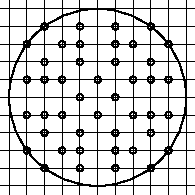
\includegraphics{taskbook-36}\\
		\footnotesize $M(5)=81$, $N(5)=44$, $\nicefrac{N}{M} = \nicefrac{44}{81}$
	\end{figure}
\end{problem}

\begin{problem}{53.}
	For the sequence of Fibonacci numbers $a_n$ from problem 43, find the limit of the ratio 
	$a_{n+1}/a_n$ when $n$ tends to infinity:\vspace{2\jot}
	\begin{equation*}
		\frac{a_{n+1}}{a_n}=2,\ \frac 32,\ \frac53, \ \frac85, \ \frac{13}8,
		\ \frac{34}{21}.
	\end{equation*}
	[The answer is \enquote{the golden ratio},
	$\frac{\sqrt{5}+1}{2\vphantom)} \approx 1.618$. This is the ratio of the sides of a card which stays
	similar to itself after cutting off the square whose side is the smaller side of the card,
	$\frac{AB}{BC}=\frac{PC}{CD}$. How is the golden ratio related to a regular pentagon and a five-pointed star?]
	\begin{figure}
		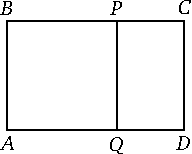
\includegraphics{taskbook-37}
	\end{figure}
\end{problem}

\begin{problem}{54.}
	Calculate the infinite continued fraction
	\begin{equation*}
		1+\cfrac{1}{2+\cfrac{1}{1+\cfrac{1}{2+\cfrac{1}{1+\cfrac{1}{2+\ldots}}}}}=
		a_0+\cfrac{1}{a_1+\cfrac{1}{a_2+\cfrac{1}{a_3+\dots}}}
	\end{equation*}
	with $a_{2k}=1$ and $a_{2k+1}=2$ (that is, find the limit of the fractions
	\begin{equation*}
		a_0+\cfrac{1}{a_1+\cfrac{1}{a_2+{\atop{\ddots \atop {}} + \cfrac{1}{a_n}}}}
	\end{equation*}
	for $n \to \infty$).
\end{problem}

\begin{problem}{55.}
	Find the polynomials 
	\begin{equation*}
		y=\cos 3 (\arccos x),\ y=\cos 4 (\arccos x),\ 
		y=\cos n (\arccos x),
	\end{equation*}
	where $|x| \leqslant 1$.
\end{problem}

\begin{problem}{56.}
	Calculate the sum of the $k$-th powers of the $n$ complex  $n$-th roots of unity.   
\end{problem}

\begin{problem}{57.}
	On the $(x,y)$-plane, draw the curves defined parametrically by: 
	\begin{equation*}
		\{x=\cos 2t, y=\sin 3t\},\quad 
		\{x=t^3-3t, y=t^4-2t^2\}.
	\end{equation*}
	\vspace{-2\baselineskip}%remove this vertical space if your translation has text coming after the equation
\end{problem}

\begin{problem}{58.}
	Calculate $\int_0^{2\pi} \sin^{100} x\,dx$ (with an error of not more than 10\% of the answer).
\end{problem}

\begin{problem}{59.}
	Calculate $\int_1^{10} x^x\,dx$ (with an error of not more than 10\% of the answer).
\end{problem}

\begin{problem}{60.}
	Find the area of a triangle with angles $(\alpha, \beta, \gamma)$ on a radius 1 sphere,
	whose sides are great circles (sections of a sphere by planes passing through its centre).

	\begin{note}{Answer:}
		$S=\alpha+\beta+\gamma-\pi$ (for example, for a triangle with 
		three right angles, $S=\nicefrac{\pi}{2}$, that is, one-eighth of the total area of the sphere).
		\begin{figure}
			\null\hfill
			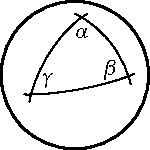
\includegraphics{taskbook-44}
			\hfill
			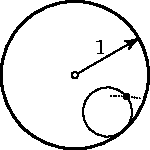
\includegraphics{taskbook-45}
			\hfill\null
		\end{figure}
	\end{note}
\end{problem}

\begin{problem}{61.}
	A circle of radius $r$ rolls (without slipping) inside a circle of radius 1.
	Draw the whole trajectory of a point of the rolling circle (this trajectory is called a hypocycloid) 
	for $r=\nicefrac{1}{3}$, for $r=\nicefrac{1}{4}$, for $r=\nicefrac{1}{n}$, and for $r=\nicefrac{1}{2}$.
\end{problem}

\begin{problem}{62.}
	In a class of $n$ pupils, estimate the probability of there being two pupils with the same birthdays. Is it high or is it low?

	\begin{note}{Answer:}
		(very) high if the number of the pupils is (well) above $n_0$,
		(very) low if it is (well) below $n_0$, and what this $n_0$ actually is
		(when the probability $p \approx \nicefrac{1}{2}$) is to be found.
	\end{note}
\end{problem}

\begin{problem}{63.}
	Snell's (Snellius') law states that the angle $\alpha$ made by a ray of light with the normal to layers of a stratified medium satisfies the equation
	\begin{equation*}
		n(y) \sin \alpha=\text{const},
	\end{equation*}
	where $n(y)$ is the refractive index of the layer at height $y$ (the quantity $n$ is	inversely proportional to the speed 
	of light in the medium when taking its speed in vacuum as 1; in water $n=nicefrac{4}{3}$).
	\begin{figure}
		\null\hfill
		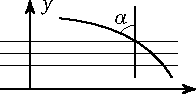
\includegraphics{taskbook-47}
		\hfill
		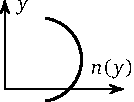
\includegraphics{taskbook-471}
		\hfill\null
	\end{figure}

	Draw ray trajectories in the medium  \enquote{air over a desert}, where the index $n(y)$ has a maximum
	at a certain height.
	(A solution to this problem explains mirages in a desert to those understanding how trajectories of rays emanating from objects are related to the images.)
\end{problem}

\begin{problem}{64.}
	Inscribe into an acute-angled triangle $ABC$ a triangle $KLM$ of minimal perimeter
	(with its vertex $K$ on $AB$, $L$ on $BC$, $M$ on $CA$).
	\begin{figure}
		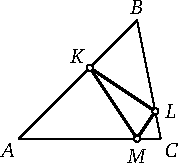
\includegraphics{taskbook-48} 
	\end{figure}

	\begin{note}{Hint:}
		The answer for non-acute-angled triangles is not similar to the beautiful answer for acute-angled ones.
	\end{note}
\end{problem}

\begin{problem}{65.}
	Calculate the mean value of the function  $\nicefrac{1}{r}$ (where
	$r^2=x^2+y^2+z^2$, $r$ is the distance to the origin) on the radius 
	$R$ sphere centred at the point $(X,Y,Z)$.

	\begin{note}{Hint:}
		The problem is related to Newton's gravitation law and Coulomb's law of electricity theory.
		In the two-dimensional version of the problem, the function should be replaced by $\ln r$, and the sphere by the circle.
	\end{note}
\end{problem}

\begin{problem}{66.}
	The fact $2^{10}=1024 \approx 10^3$ implies
	$\log_{10} 2 \approx 0.3$. 	Estimate how much they differ, and calculate $\log_{10} 2$ to three decimal places. 
\end{problem}

\begin{problem}{67.}
	Find $\log_{10} 4$, $\log_{10} 8$,
	$\log_{10} 5$, $\log_{10} 50$, $\log_{10} 32$, $\log_{10} 128$,
	$\log_{10} 125$, $\log_{10} 64$ with the same precision.
\end{problem}

\begin{problem}{68.} 
	Using $7^2 \approx 50$, find an approximate value of $\log_{10} 7$.
\end{problem}

\begin{problem}{69.}
	Knowing $\log_{10} 64$ and $\log_{10} 7$, find $\log_{10} 9$, $\log_{10} 3$,
    $\log_{10} 27$, $\log_{10} 6$, $\log_{10} 12$.
\end{problem}

\begin{problem}{70.}
	Using $\ln (1+x) \approx x$ ($\ln$ is $\log_e$), find $\log_{10} e$ and
    $\ln 10$ from the relation\footnote{The Euler number $e = 2{.}71828\dots$ is defined as the limit of the sequence
	$\left(1+\frac{1}{n}\right)^n$ for $n\to \infty$, and is equal to the sum of the series 
	$1+\frac{1}{1!} +\frac{1}{2!}+\frac{1}{3!}+\dotsb$. It may also be defined via the quoted formula for 
	 $\ln (1+x)$: $\lim\limits_{x\to 0}\frac{\ln(1+x)}{x} = 1$.}
	%
	\begin{equation*}
		\log_{10} a=\frac{\ln a}{\ln 10}
	\end{equation*} 
	and from the values of $\log_{10} a$ calculated earlier (for example, for $a=128/125, 1024/1000$
	and so on).

	[Solutions to problems 65--69 deliver after half an hour a table of four-digit logarithms of any numbers using
	products of numbers found already as basic data and the formula  
	\begin{equation*}
		\ln (1+x) \approx x-\frac{x^2}{2}+\frac{x^3}{3}-\frac{x^4}{4}+\dotsb,
	\end{equation*}
	for corrections.] (In this way Newton compiled a table of
	40-digit logarithms!)
\end{problem}

\begin{problem}{71.}
	Consider the sequence of powers of two: $1$, $2$, $4$, $8$, $16$, $32$, $64$,
	$128$, $256$, $512$, $1024$, $2048, \dotsc$ Among the first twelve numbers, four have their decimal expression
	starting with 1, and none has it starting with 7.

	Prove that in the limit $n \to \infty$ the first digit of the numbers $2^m$,
	$0\leqslant m \leqslant n$, will be met with a certain frequency:
	$p_1 \approx 30\%, p_2 \approx 18\%, \dotsc, p_9 \approx 4\%$.
\end{problem}

\begin{problem}{72.}
	Verify the behaviour of the first digits of powers of three: $1,
	3, 9, 2, 8, 2, 7, \dotsc$ Prove that, in the limit here, we also 
	get certain frequencies and, moreover, the same as for the powers of two.
	Find an exact formula for $p_1, \dotsc, p_9$.

	\begin{note}{Hint:}
		The first digit of a number $x$ is determined by the fractional part
		of the number $\log_{10} x$, therefore one has to consider the sequence of the fractional parts of
		the numbers $m \alpha$, where $\alpha=\log_{10} 2$.
	\end{note}
	Prove that these fractional parts are distributed over the interval from 0 to~1
	uniformly: out of the $n$ fractional parts of the numbers $m \alpha$, $0 \leqslant m<n$,
	a subinterval $A$ will contain the quantity~$k_n (A)$ such that, for $n \to \infty$,
	$\lim (k_n (A)/n)=(\text{the length of the subinterval~$A$})$.
\end{problem}

\begin{problem}{73.}
	Let $g\colon M \to M$ be a smooth map of a bounded domain $M$ onto itself which
	is one-to-one and preserves areas (volumes in the multi-dimensional case) of domains.

	Prove that in any neighbourhood $U$ of any point of $M$ and for any $N$ there exists a point $x$
	such that $g^T x$ is also in $U$ for a certain integer $T>N$ (\enquote{the recurrence theorem}).
\end{problem}

\begin{problem}{74.}
	Let $M$ be the torus surface (with coordinates $\alpha \pmod{2\pi}$, $\beta \pmod{2\pi}$), 
	and
	\begin{equation*}
		g(\alpha, \beta)=(\alpha+1, \beta+ \sqrt{2}) \pmod{2\pi}.
	\end{equation*}
	Prove that the sequence of points
	$\{g^T (x)\}$, $T=1, 2, \dotsc$, is everywhere dense in the torus.
\end{problem}

\begin{problem}{75.}
	In the notation of problem 74, let
	\begin{equation*}
		f(\alpha, \beta)=(2\alpha+\beta,\alpha+\beta) \pmod{2\pi}.
	\end{equation*}
	Prove that there is an everywhere dense subset of the torus consisting of periodic points $x$ (that is, such that 
	$f^{T (x)} x=x$ for certain integer $T>0$).
\end{problem}

\begin{problem}{76.}
	In the notation of problem 74 prove that, for almost all points $x$ of the torus,
	the sequence of points $\{g^T (x)\}$, $T=1, 2, \dotsc$, is everywhere dense in the torus
	(points $x$ without this property constitute a set of measure zero).
\end{problem}

\begin{problem}{77.}
	In problems 74 and 76 prove that the sequence $\{g^T (x)\}$, $T=1, 2, \dotsc$, is distributed
	over the torus uniformly: if a domain $A$ contains $k_n(A)$ points out of the $n$ with $T=1, 2, \dotsc,n$, then
	\begin{equation*}
		\lim_{n \to \infty} \frac{k_n(A)}{n}=\frac{\operatorname{mes} A}{\operatorname{mes} M}
	\end{equation*}
	(for example, for a Jordan measurable domain $A$ of measure $\operatorname{mes} A$).
\end{problem}

\vfill
\begin{note}{Note to problem 13.}
	I tried to illustrate with this problem the difference in approaches to tasks by mathematicians and physicists, in my invited paper in the journal \enquote{Physics -- Uspekhi} for the 2000 Christmas jubilee. My success surpassed by far what I intended: the editors, unlike preschoolers, on whom I had been basing my experience, failed to solve the problem, and therefore altered it to match my \SI{4}{\mm} answer as follows: instead of \enquote{from the first page of volume 1 to the last page of volume 2} they typeset \enquote{from the \emph{last} page of volume 1 to the \emph{first} page of volume 2}.

	This true story is so implausible that I am including it here: the proof is the editors' version published by the journal.  
\end{note}
\clearpage
\null\vfill
\noindent
Translation Russian - English:\\
\null\quad Victor Goryunov and Sabir Gusein-Zade\\
\\
Design and layout:\\
\null\quad Konrad Renner and Christian Stussak\\
\\
\\
From the Russian edition:\\
\null\quad \textrussian{В. И. Арнольд: Задачи для детей от 5 до 15 лет}\\
\null\quad Moscow, MCCME, 2004\\
\null\quad ISBN 5-94057-183-2\\
\\
\\
Picture credits title page:\\ 
\null\quad Archives of the Mathematischen Forschungsinstituts Oberwolfach\\
\\
Version:\\
\null\quad \today\\
\\
This book is available under the CC BY-NC-SA 3.0 license at the IMAG\-I\-NARY platform: \href{http://www.imaginary.org/background-materials}{www.imaginary.org/background-materials}.\\
IMAGINARY is a project by the Mathematisches Forschungsinstitut Oberwolfach supported by the Klaus Tschira Stiftung.
\end{document}
